
\chapter{基于硬件事务内存的并发哈希表的实现}

%备选标题:基于RTM的锁省略算法
\section{事务内存的基本概念}
事务内存(TM)是一种简化并发编程的并发控制范式,其源自于数据库管理系统中的事务概念。
它的核心思想是将一段代码标示成一条事务。
在数据库管理系统中,事务必须满足ACID性质,即原子性(Atomicity)、一致性(Consistency)、隔离性(Isolation)和持久性(Durability)。
原子性指的是事务中的动作要么全部执行,要么一个都不执行;一致性指的是任何时刻,数据库必须处于一致性状态,即必须满足某些预先设定的条件;隔离性是指一个事务不能看见其它未提交事务所涉及到的内部对象的状态;而持久性则是指一个已提交的事务对数据库系统的改变必须是永久的。

事务内存继承了事务的ACID原则。
事务内存的原子性是指事务代码区间的内容要么全部执行,要么全部不执行,不存在有事务代码停滞在中间的任何一条语句,如果发生意外而中止了事务,则系统状态会回滚到事务起始的状态继续执行;
事务内存的一致性是指是指事务应该要么执行完成并令外界看到其造成的变化,要么执行失败并使所有相关状态都保持不变。如果有多个事务同时运行,那么从这些事务之外的角度来进行观察,它们对系统状态做出的改变始终是一个接着一个发生的,中间不会有任何交叉。例如,在(对同一个账户)两个独立且并发的存款和取款事务完成之后,账户余额应该是两个操作所产生的累加效果(取钱是对账户加上一个负数)。
事务内存的隔离性是指并发执行的多个事务代码区间彼此之间是严格隔离的,本事务无法了解其他事务的局部变更结果,所有事物造成系统状态的变化只有在成功提交之后才对外部可见;
事务内存的持久性是指事务代码执行完成成功提交之后,对于系统状态的变更是持久有效的,并不会回退到起始状态,直到有新的事务执行的代码改变这个状态。

事务内存具有两个重要的性质,即事务内存要确保对临界区代码片段的执行具有原子性和隔离性。
满足原子性和隔离性的事务内存可以安全的并行执行,可以取代现有的令人头疼的锁机制与原子原语。
基于锁的并发编程是一种悲观的并发模式,它假设获得锁的线程一定会访问共享数据,从而会对其他线程进行阻塞。
而任意两条访问加锁的变量的事务能够并发的执行,并且只有在其中一条事务尝试修改共享数据时触发回滚。

事务内存被认为是最有希望解决多核处理器编程问题的并发编程方案之一。
它最吸引人的特点是程序员只需在本地对共享数据的访问进行推理,并让底层系统确保正确的并发执行。
该模型有望提供细粒度锁机制那样的线程扩展性并能避免由一般的锁机制中常见的陷阱,比如死锁等问题。

本章主要研究硬件事务内存对构建并发哈希表的作用。

\section{Intel事务同步扩展}
2012年2月,Intel发布了其支持硬件事务内存的事务同步扩展(Transactional Synchronization Extensions, TSX),并于2013年6月在其基于Haswell微体系结构的微处理器上亮相。
标志着硬件事务内存的全面商用化。

TSX对使用锁锁省音方式编写的多线程并发软件具有明显的加速所用。 
TSX提供一组扩展指令集,允许编程人员指定事务同步的代码区域。
有了事务同步,硬件就能动态的决定线程是否需要对锁保护的临界区进行串行化,并且只在必要的时候执行串行化。
这允许处理器利用由于动态的不必要的同步而隐藏起来的并发性。
在Intel TSX的最底层,编程人员指定的代码区域(也称为事务区域)就能事务性的执行。
如果事务执行成功完成,那么对其他逻辑核而言所有在事务区间执行的内存操作都像是在瞬间发生的。
只有确认成功提交后,在执行事务区域期间对于系统的更新操作才会对其他逻辑核可见,该过程称为一次原子提交。
这样,编程人员只需使用粗粒度的锁编程就能实现细粒度锁的性能。
如果多个线程同时访问受同一个锁保护的临界区而彼此之间有不存在任何数据冲突,那么这些线程就能并发的执行而无需串行化。

Intel TSX提供两种不同的软件接口。
一种称为硬件锁省略(Hardware Lock Elision,HLE);一种称为限制性事务内存(Restricted Transactional Memory,RTM)。

\subsection{Intel硬件锁省略}
HLE提供与传统指令集兼容的指令集接口供编程人员编写事务化的程序,还提供两条全新的指令前缀XACQUIRE和XRELEASE。

使用HLE时,将XACQUIRE前缀放置在用于获取保护临界区的锁的指令的前面。
处理器将XACQUIRE视为省略写相关的锁获取操作的提示。
即使是获取锁的请求与该锁有关联的写操作,处理器也不会将锁的地址添加到事务区域的写集中而是将锁的地址添加到事务区域的读取集中,更不会向该锁发起任何写入请求。
之后逻辑处理器进入事务执行。
如果在XACQUIRE前缀指令之前是可用的,那么后面的其他所有的处理器都将该锁视作是可用的。
因为当前正在事务化执行的逻辑处理器不会将锁的地址写入到它的写集中,也不对其执行外部可见的写操作,其他的逻辑处理器仍然可以读取该锁而不会造成数据冲突。
这就允许其他的逻辑处理器也进入并且并发的对受同一个锁保护的临界区进行操作。
处理器将自动检测事务执行期间发生的任何数据冲突,有必要时执行中止事务操作。

XRELEASE前缀放置在用于释放保护临界区的锁的指令的前面。这涉及到对锁的写的问题。
如果XRELEASE正在试图将锁的值恢复到XACQUIRE发起锁请求时所操作的同一个锁的值,那么处理器将省略所有与即将释放的锁相关的所有外部锁请求并且该锁的地址不会被添加到写集中。
然后处理器尝试提交事务执行。

使用HLE时,有多个线程同时执行到被同一个锁保护的临界区时,如果它们执行的操作不会相互之间产生数据冲突的话,这些线程可以并发执行。
如果无法事务的执行代码区域,处理器将不使用省略而以普通的方式执行代码区域。
HLE确保软件有与基于锁的非HLE模式相同的前向执行的能力。
对于一次成功的HLE执行,锁和临界区代码都必须遵循特定的指导原则~\cite{Intel2015Intel}。
这些指导原则将会对性能产生影响,不遵循这些指导原则不会造成功能性的失败。

不支持HLE的硬件会忽略掉XACQUIRE和XRELEASE前缀提示,也不会执行任何省略操作。
更为重要的是,HLE很好的与现有的基于锁的编程模型兼容。
在基于锁的编程模型中不正确的使用XACQUIRE和XRELEASE前缀提示不会引起功能错误,但它可能会暴露代码中已经存在的潜在的漏洞。

\subsection{Intel限制性事务内存}
RTM为事务的执行提供了更为灵活的接口。
它提供三条新的指令——XBEGIN, XEND和XABORT——供用户启动,提交和中止一次事务执行。

XBEGIN指令用于指定事务代码区域的起始位置,XEND指令表示事务代码区域的结束。
XBEGIN指令携带一个操作数,该操作数用于表示到回滚指令地址的相对偏移量,如果RTM代码区域无法成功的进行事务化执行,将会推到该操作数指向的指令继续执行。

处理器有很多原因中止RTM的事务执行。
硬件自动检测事务中止条件,退回到回滚指令处以从XBEGIN开始的指令时的体系结构状态和EAX寄存器更新的描述事务中止的状态重新开始执行。

XABORT指令允许用户显示的中止RTM代码区域的执行。
它携带一个8位的直接参数,这个参数被加载到EAX寄存器中并将在发生RTM中止后对软件可见。具体参数的意义见表~\ref{tab:rtm_status}~。

\begin{table}[htbp]
  \centering
  \caption{RTM的中止状态定义}
  \label{tab:rtm_status}
  \begin{tabular}{cc}
    \toprule
       EAX寄存器比特位 & 说明 \\
    \midrule
      0     & 由XABORT指令引起的中止 \\
      1     & 该事务有可能在Retry之后成功\\
      2     & 该次中止是因数据冲突而引起的 \\
      3     & 该次中止是因内部的缓存溢出引起的\\
      4     & 该次中止是因调试断点引起的 \\
      5     & 该次中止是因事务嵌套引起的 \\
      23:6  & 保留位\\
      31:24 & XABORT参数(只有位0被置位时有效) \\
    \bottomrule
  \end{tabular}
\end{table}

RTM指令没有任何与它们相关联的数据存储位置。
虽然硬件无法保证RTM区域总是能够成功地进行事务地提交,但大多数遵循推荐指南的事务都有望成功地进行事务处理。
然后,用户必须在回退路径中提供备选的代码序列,以确保程序的前向执行。
比如,通过简单的锁申请然后以非事务的方式执行制定的代码区域。
此外,总是在特定的实现中发生中止的事务可能会在接下来的实现中完全事务的执行。
因此,用户必须确保事务性区域代码的路径和备选代码序列在功能上是完备的。

使用Intel RTM必须获得相应的硬件支持,在不支持RTM的平台上无法完成编译。
这是RTM有别于HLE的地方之一。

\subsection{TSX的Lemming效应}
\textit{Lemming}效应是指正在运行中的事务之间陷入一种相互阻扰对让进入事务执行的状态。
具体的,任意获得锁的线程会对锁变量进行修改同时强制其他当前正在该锁上执行锁省略过程的线程中止。
这些被中止的线程随后会尝试重新尝试事务的执行或者尝试获取锁。
当存在多个线程都处于这一过程时,这些线程会陷入一种持续阻挠对方回退到回退路径的状态,使得锁省略过程长时间停滞。

被省略的锁有一个强制的惯例,即要么所有的锁用户都是省略的,要么所有的锁用户都是真实的持有锁。
一般的情况下总是这样,除了一些特殊的情况可以避免这种惯例。
这种惯例确保对任何实际持有锁的线程执行正确的锁语义。

在HLE中,受锁保护的代码段执行时通过启动一条事务并假装“获取”锁但实际上并没有真正持有该锁。
也就是说,锁被读取,如果它的状态被解锁,那么它就被放置在被锁住的事务读集中,而不影响锁的状态,这仍然保持解锁状态。
然而,当事务中止时(例如发生冲突),它会执行回滚然后以非推测性的方式获取锁,并将锁写入。
被中止的线程获取的全局可见的锁与执行推测运行的HLE事务时推测性加载的锁发生冲突,由于在锁的位置上发生了冲突,所以会导致所有这些锁被中止。此外,当新的线程到达临界区时发现当前锁已经被其他线程持有时,新的线程不会启动它们的事务。
在公平锁的情况下,获取锁时的冲突会使得线程无法并行的执行,这种情况一直会持续到经历一个没有线程试图访问锁的静默期为止。
这种引起不必要的串行化从而限制并发度的现象称为\textit{Lemming}效应~\cite{Dice2008Applications}。

当中止率升高时,\textit{Lemming}效应的影响会越来越严重。
如果是在中止率很低的情况下,\textit{Lemming}效应的影响可以忽略不计。
从本质上说,\textit{Lemming}效应使得事务从中止中恢复过来的成本更高,并且引起不必要的序列化执行。

在事务的执行过程中,常常由于冲突而导致事务中止。
事务申请获取的锁当前被其他线程占有从而被迫中止,但是占有该锁的线程可能很快执行完成并释放锁。
因此,大部分被中止的事务经过一次或者多次重试之后可以成功获取锁,完成提交。
Intel在TSX开发者手册中提倡使用RTM进行锁省略编程时适当的进行RTM重试有助于提升性能。
使用RTM编写锁省略代码时,如下行为会引起\textit{Lemming}效应的加剧:

\textbf{第一,过快的进行RTM重试。}当检测到发生中止时立即进行重试。
考虑这么一种情况,设定最大重试次数为5次(重试5次仍然无法成功提交则方式事务执行转而使用常规方式申请锁执行),假设现在有t$_1$和t$_2$两个线程在并行的执行事务代码,t$_1$长时间的持有锁。
这时t$_2$尝试申请锁,但发现当前锁不空闲,于是立即开始重试,重试次数很快达到5次,此时t$_1$仍然没有释放锁,t$_2$回滚,然后使用标准方式申请锁完成执行。
如果有更多的线程并行的处于上述状态,它们将陷入\textit{Lemming}效应的魔咒。
这些重试达到最大次数进入回滚路径执行的线程排队等待锁执行,长时间无法再一次进入到事务执行。
对性能造成损耗。

\textbf{第二,设定的RTM重试次数过大。}一般的,在使用RTM进行锁省略编程时通常能够提升性能。
而且,对于不同的工作负载最大重试次数是弹性变化的。
但是,当设定的重试次数过大时,会有加剧运行其他工作负载的\textit{Lemming}效应的风险。
同样以t$_1$和t$_2$为例,假设t$_1$和t$_2$都尝试事务执行,它们运行临界区,一定的时间后同时造成对方中止。
然后,它们进行重试,又一次遇到上述情况,如此循环若干次。
摆脱这种纠缠不清的状态的方法是其中一方进去到回退路径申请标准锁执行。
但是,如果重试次数过高,它们在进入回退路径之前会浪费较长的时间。

\textbf{第三,不设定回退路径,不停的进行重试。}除了冲突可能造成事务中止之外,还有其他原因(比如执行TSX不兼容的指令,动态连接库,页脏位以及其他异常等)也会造成中止,TSX不能保证每次事务执行都能成功。
不设置回退路径可能导致程序挂起。

\textbf{第四,没有将锁变量放入读集合内。}锁省音依赖于其读集合中的锁变量,用来确保推测行执行和真实的锁持有者之间的完全同步。
这要求在事务执行过程中至少读取一次锁变量。
如果该锁只使用单一的锁变量,那这个过程将由HLE自动完成,但是当锁有多个锁变量的时候,即便是有HLE的的情况下,这个过程也可能会出错。

\textbf{第五,在事务执行完成时使用\textit{xtest}代替锁的状态检测。}

\section{软件优化的硬件锁省略技术}

在使用硬件事务内存设计并发哈希表时,为了减轻
\textit{Lemming}效应对性能造成的负面影响,Intel的开发者手册中建议对被中止的事务进行重试~\cite{Intel2015Intel}。
然而,从上一节中关于触发\textit{Lemming}效应的原因中得知,过快、过度的使用RTM重试或者不对RTM重试的次数做出限定同样会引起\textit{Lemming}效应。
Y. Afek等人通过实验也表明这种简单的技术方案并没有完全缓解这个问题~\cite{Afek2014Software},尤其是当\textit{Lemming}效应很严重时,比如使用公平锁或者高并发度情况下,单纯的依靠使用RTM重试不能有效缓解\textit{Lemming}效应的副作用。
为了有效的抑制\textit{Lemming}效应造成的性能下降问题,他们提出了两种软件辅助的优化方案:软件优化的硬件锁删除方法和软件辅助的冲突检测方法。

\subsection{软件辅助的硬件锁删除方法}
软件辅助的锁删除技术,Software-assisted lock removal (SLR),是为了克服Lemming效应的影响,引入的第一种方法。
这种方法可以视为对Rajwar和Goodman~\cite{Rajwar2002Transactional}硬件锁删除技术的软硬件混合实现。
Rajwar和Goodman观察到只要事务内存能够为冲突的事务提供前向保证,那么就可以不需要锁执行具有相同临界区的事务(也就是通过启动事务代替申请锁,提交事务代替释放锁)。
然而,Haswell的硬件事务内存使用非常简单的“请求者至上”的冲突解决策略~\cite{2011Intel},而这一策略容易引起“活锁”~\cite{Bobba2007Performance}。

\SetKwProg{Fn}{Function}{}{}
\begin{algorithm}[htbp]
\SetAlgoLined
\Fn{lock()}{
  $retries \gets $ 0 ~~\\
  // speculative path~~\\
  XBEGIN (line 6)   \tcc*[f]{如果发生中止,跳转到第6行重试}\; 
  \Return
  ~~\\
  // fallback path~~\\
  $retries \gets retries + $ 1 ~~\\
  \eIf{$retries < MAX\_RETRIES $}{
    goto Line 3
  }{
    lock.lock() \tcc*[f]{执行标准锁请求}
  }
}
\caption{SLR的加锁方法}
\label{algo:slr_lock}
\end{algorithm}

SLR方案使用如下方法避免上述提到的问题,其加锁和解锁过程如算法~\ref{algo:slr_lock}~和~\ref{algo:slr_unlock}~所示。
在算法~\ref{algo:slr_lock}~中,第3行标示事务代码区域的起始位置,如果发生中止,则跳转到第6行尝试再一次的以事务的方式执行,如果重试的次数超过预先限定的门限值MAX\_RETRIES,则放弃事务执行,转而用普通的方式通过申请锁完成本次执行(第10行)。

\SetKwProg{Fn}{Function}{}{}
\begin{algorithm}[htbp]
\SetAlgoLined
\Fn{unlock()}{
   \eIf{$ XTEST() $}{ \tcc*[f]{如果本次为事务执行,返回TURE}~~\\
      \eIf{lock is $ TRUE $}{
          XABORT       \tcc*[f]{中止事务执行}
      }{
          XEND
      }
   }{
      lock.unlock()   \tcc*[f]{以标准解锁方式解锁}
   }
}
\caption{SLR的解锁方法}
\label{algo:slr_unlock}
\end{algorithm}

SLR使用HTM在不访问锁的情况下事务的执行临界区,直到准备提交。
如果当前锁未被其他线程持有,则SLR读取锁并提交;否则的话发生事务中止并重试。
重试多次之后仍然失败,此时SLR会放弃事务的执行转而以非事务的(常规的)方式申请锁完成该次操作。
在SLR中,获取锁的线程不会自动与运行事务冲突,也不会阻止到达的线程以推测的方式启动事务。
因为在SLR中,推测的事务可能并发的运行到持有锁的事务中,此时推测事务可能看到不一致的状态(这将确保推测事务提交失败然后中止)。

\subsection{软件辅助的冲突检测方法}

算法~\ref{algo:scm_lock}~和~\ref{algo:scm_unlock}~描述了SCM的加锁和解锁的过程。

\SetKwProg{Fn}{Function}{}{}
\begin{algorithm}[htbp]
\SetAlgoLined
\Fn{lock()}{
  $retries \gets 0$ \; 
  \tcc{primary path}~~\\
  XBEGIN (line 6)   \tcc*[f]{如果发生中止,跳转到第6行重试} ~~\\
  条件成熟时调用HLE或者SLR的$lock()$方法\;
  \Return
  ~~\\

  \tcc{serializing path}~~\\
  \eIf{aux\_lock\_owner  is $ FALSE $}{
      $ retries \gets retries + $1\;
  }{
      aux\_lock.lock()      \tcc*[f]{辅助锁申请锁}~~\\
      $aux\_lock\_owner \gets TURE$
  }
  \eIf{ $retries < MAX\_RETRIES $}{
      goto Line 3
  }{
      main\_lock.lock()
  }
  }
\caption{SCM的加锁方法}
\label{algo:scm_lock}
\end{algorithm}

软件辅助冲突管理技术(Software-assisted Conflict Management, SCM)。
SLR方法虽然能够很好的抑制\textit{Lemming}效应,但是以损失不透明度为代价。
SCM是另一种抑制\textit{Lemming}效应的软件辅助方法。
SCM是一种简单的冲突管理技术,它允许不冲突的线程继续运行其推测性的基于HLE的事务,而不受产生冲突的线程的影响。
为此,在锁的实现中添加一个串行化的路径,其中一个被中止的线程必须获得一个独立的辅助锁(不使用锁省略)以便重新加入与其他线程的推测执行。使用这种方法,发生冲突的线程之间被串行化,而不影响其他线程的并行执行。
如果线程在多次冲突中失败,那么它必须放弃推测执行转而申请原始锁。


SCM方法使用了两种锁,一种为主锁(\textit{main\_lock}),一种为辅助锁(\textit{aux\_lock})。
主锁使用的是HLE/SLR机制中的一种,而辅助锁是一种标准的传统锁。
只有在以标准的非事务执行方式执行代码区域时才会申请使用辅助锁(算法~\ref{algo:scm_lock}~第9、10行)。
辅助锁会将所有陷入冲突的线程召集到一起,然后将它们串行化的执行。
当某一事务被中止时,被中止的线程以非事务性的方式申请辅助锁,随后重新加入到对原始临界区的推测执行队列中。
这种为了重新加入到推测执行队列而申请辅助锁的过程称为串行化的路径(serializing path)。
线程在进入串行化路径之前会对事务进行重试。

\SetKwProg{Fn}{Function}{}{}
\begin{algorithm}[htbp]
\Fn{unlock()}{
\eIf{XTEST()}{
  调用HLE或者SLR的$unlock()$方法
  XEND
}{
  main\_lock.unlock()
}
\If{$ aux\_lock\_owner = TRUE $}{
  aux\_lock.unlock() ~~\\
  $aux\_lock\_owner \gets FALSE$
}
}
\caption{SCM的解锁方法}
\label{algo:scm_unlock}
\end{algorithm}
SCM和SLR也可以结合起来进一步减少当SLR线程放弃并以非事务的方式申请锁时引起的任何前向问题。

上述的两种软件辅助方法已经使用标准的pthread锁接口封装到动态库中。
可以直接在程序中使用上述方法而无需对代码进行调整,也无需重新编译。


\section{基于HTM的并发哈希表的设计}

\subsection{问题引入}

%哈希表操作示意图
\begin{figure}[htbp]
\centering
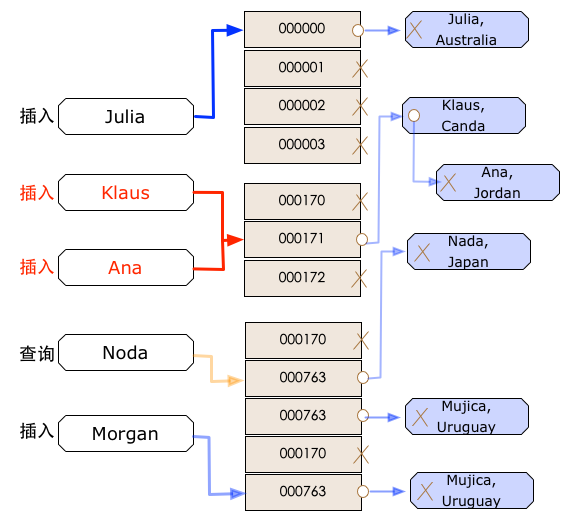
\includegraphics[width=0.9\textwidth]{hashtable}
\caption{串行执行五个操作的哈希表}\label{fig:hashtable}
\end{figure}

哈希表用于在线性时间内对键和键值对之间建立映射关系。
插入和查询是哈希表的两种核心操作,当然哈希表的扩张和删除操作也很重要,但是这里为了简要的引出我所要解决的问题,暂时不考虑哈希表的扩张和删除操作。

考虑这么一种场景,有一个简单的如图~\ref{fig:hashtable}所示哈希表,它串行的执行五次操作,分别是插入、插入、插入、查询、插入。
现在变更需求,希望将这个哈希表设计成并发的,会有怎样的问题呢?

设计高并发的哈希表并不是一件简单的事,目前有很多方法,比如基于锁的方法,使用原子指令实现的无锁化编程等,用于构建高并发度的并发哈希表。
但是这些方法无疑都会涉及到更加复杂的数据结构的设计,同时也增加了程序的复杂性。

使用粗粒度锁方法(全局锁,只用一把锁)实现并发是最简单的方法。
具体的方法是将整个哈希表作为临界区,只用一个锁对临界区进行保护。
在这个方法中,每一次对哈希表的操作都是先申请锁,然后执行相应操作,再释放锁。
当前锁被其他线程持有时,其他线程无法获得锁,因此也不允许对哈希表进行其他操作。
显然,这种方法的缺陷是致命的,它的效率非常低。

现在尝试细粒度的锁方法。具体的方法是将哈希表分成更小的区间,每个区间用一个锁保护。
也就是缩短了临界区的长度。使用这种方法的好处是,可以允许多个线程在不存在数据竞争的前提下并发的对哈希表进行操作。
相比于之前采用的整个哈希表用一把锁的情形,显然细粒度锁方法的效率要更高。
但是细粒度锁方法同样也存在缺陷,它引入了不必要的延迟,并且使得数据结构的设计更加复杂,且难以保证正确性。

粗粒度锁方法易用,便于理解,易于调试,唯一的缺陷是在多线程环境下对性能造成阻碍。
在多处理器上这个缺陷是致命的,不可调和的。
细粒度锁方法能够较好的发挥多核处理器的性能,但是细粒度锁方法的实现方式复杂,且正确性难以得到保障。
那是否有一种方法既具备粗粒度锁方法易用,便于理解,易于调试的特点,又具备细粒度锁方法的性能呢?
有!Intel TSX很完美的具备了两种方法的长处,对于并发数据结构的设计具有重要意义。

图~\ref{fig:hashtable}~中的五个操作,只有两个插入操作存在冲突。
其他的三个操作都是互不干扰的。因此,在全局锁的上使用HLE可以完全的将锁省略掉。
换句话说,使用这种方法获得的性能与执行没有加锁和解锁过程的代码获得的性能非常接近。
造成性能相近的关键原因是这些操作受到Intel TSX的保护,该硬件取代了锁的功能,悄无声息的完成了对临界区的保护。

至于被映射到同一地址的两个操作由于存在冲突,所以需要交错执行。
但是,在多线程环境中,两个操作有可能被两个线程同时执行。
Intel TSX将确认在这种情况下确实需要加锁以保证代码的正确执行,同时也会因为加锁操作而引入额外的开销。
实际上,出现这种情形时,相互冲突的任务将执行到事务代码里面,一直到处理器检测到了这个冲突。
这时,双方都会中止事务代码的执行。
最常用的解决这个问题的方法是让每个任务继续以非事务的方式(常规的获取锁,释放锁的方式)执行。
这就意味着,总有一个任务先获得锁而进入临界区完成操作,而另一个任务则延迟直到先进入临界区的任务执行完毕。


\subsection{缓存行哈希原型描述}

\SetKwProg{Fn}{Function}{}{}
\begin{algorithm}[htbp]
\SetAlgoLined
\SetKwRepeat{Do}{do}{while}%
\SetKwFunction{Insert}{Insert}%
\Fn{Insert(hashtable,key,val)}{
  初始化\;
  $lock \gets \&bucket\rightarrow lock$\;
  $empty \gets NULL$\;
  $empty\_v \gets NULL$\;
  LOCK\_ACQ(lock)\;

  \While{True}{
  \For{$j=0$ \KwTo $ENTRIES\_PER\_BUCKET - 1$}{
    \If{$\&bucket\rightarrow key[j] == key $}{
      LOCK\_RLS(lock)\;
      \KwRet {$false$}\;
    }
    \ElseIf{$empty == NULL $ and $bucket.key[j] == 0$}{
      $empty \gets \&bucket\rightarrow key[j]$\;
      $empty\_v \gets \&bucket\rightarrow val[j]$\;
    }
  }

   \If{$bucket\rightarrow next == NULL$}{
      \eIf{$empty == NULL$}{
       $bucket\rightarrow next \gets clht\_bucket\_create()$\;
       $bucket\rightarrow next \rightarrow key[0] \gets key$\;
       $bucket\rightarrow next \rightarrow val[0] \gets val$\;
      }{
       $\*empty\_v \gets val$\;
       $\*empty \gets key$\;
     }

     LOCK\_RLS(lock)\;
     \KwRet{$true$}\;
  }
  $bucket \gets bucket\rightarrow next$\;
  }
}
\caption{CLHT-lb的插入方法}
\label{algo:clht-lb-insert}
\end{algorithm}

经过第~\ref{chap:chts}中对现有并发哈希表的深入评估与分析之后,发现缓存行哈希在多个平台上无论是线程扩展性、性能或者延迟这些方面都具有突出的表现。
因此,在设计基于硬件事务内存的并发哈希表时,参考了缓存行哈希表的数据结构的设计思路。

在前一章的内容中详细介绍了缓存行哈希表(第\ref{sec:clht}节)的设计思想、原理以及同步方法。
这里再就与本章内容密切相关的内容做一个简单的回顾。
\textcolor{red}{缓存哈希的哈希桶被设计成具有与主流计算机缓存行相同的大小(64字节)。
每一个哈希桶中包含了一个8字节的同步控制字段,用于存放锁(用于实现基于锁的版本)或原子快照(用于实现无锁版本的同步控制)。
基于锁的缓存行哈希表采用细粒度锁(每个哈希桶都有一个锁字段)完成对读者和写者的同步控制。
查询操作遍历键/值对,如果匹配,则返回值。
算法~\ref{algo:clht-lb-insert}~描述了基于锁的缓存行哈希表的插入操作的过程。
更新操作首先需要执行进行一次查询以确定该操作可以继续执行(如果插入元素时发现桶内已存在相同元素或者删除元素时发现桶内没有该元素则不进行下面的操作),如果可以继续执行,则持有该桶的锁,直到完成相应的更新操作,完成后释放锁。
如果当前映射到的哈希桶内已经没有足够的空间插入新的元素,则会选择使用指针字段链入一个新的哈希桶,或者触发哈希表扩张操作(resize)。
}

由于缓存行哈希表在设计时遵循最小化缓存行切换的原则,并通过细粒度锁方式使得临界区的长度固定为一个缓存行大小。
这就使得它具有一个天然的优势,所有的操作至多只需要一次缓存行切换就能完成。
这样可以避免单次操作过多的缓存未命中次数对系统性能的消耗。
所以在对其进行评估与分析时,它具有优于其他并发哈希方法的性能。
通过评估的结果还发现缓存行哈希表对NUMA架构的多核系统有好,能够很好的克服访问远程结点开销过高的问题。

但是,缓存行哈希表同样存在一些不足之处:

第一,较之Cuckoo、Hopscotch等哈希表,缓存行哈希表需要消耗更多的内存。这主要体现在两个方面:
\begin{itemize}
\item 基于链表的实现方法占用更多的内存空间。使用链表组织哈希桶的结构可以保证查询速度以及哈希表的空间利用率,但是每个桶都需要有8字节用于存放指针;
\item 以缓存行大小为粒度的锁实现消耗更多内存。临界区的长度等于一个缓存行的大小,每个哈希桶都包含8字节的信息用于并发控制(锁版本该位置存放锁,无锁版本该位置存放的是原子快照)。
\end{itemize}

第二,细粒度锁方法虽然能够保证线程扩展性以及稳定的性能,但其实现复杂度过高并且正确性得不到保证。

硬件事务内存为多线程应用的同步提供硬件指令支持,使用硬件事务内存既可以实现无锁化编程,又能用于实现锁。
它以粗粒度的锁实现达到或者接近使用细粒度锁方法所获得的性能。
本文以基于锁的缓存行哈希表为基础,使用Intel RTM实现基于硬件事务内存的并发哈希表。
并运用SLR和SCM两种技术用于优化RTM实现的锁以获取更高的性能。

\subsection{基于软件优化方法的加锁和解锁描述}

\subsubsection{加锁过程}

\SetKwProg{Fn}{Function}{}{}
\begin{algorithm}[htbp]
\SetAlgoLined
\Fn{lock\_mutex\_lock(*mutex)}{
  $*lock \gets  *mutex$\;
  $reason \gets 0$\;
  speculative\_path:~~\\
  XBEGIN(fallback\_path, reason)\;
  \KwRet {$0$}\;

  fallback\_path:~~\\
  $retries \gets retries + 1$\;
  \If{$retries < MAX\_RETRIES$}{
    goto speculative\_path\;
  }
  $*prev \gets NULL$\;
 
  \eIf{$thread\_handle == lock\rightarrow aux\_lock\_owner$}{
    $lock \rightarrow aux\_retries++$
  }{\tcc{以标准方式申请辅助锁}
    $my\_aux\_node.locked \gets true$\;
    $prev \gets \_\_sync\_lock\_test\_and\_set(\&lock\rightarrow aux\_lock, \&my\_aux\_node)$\;
    \If{$prev != NULL$}{
      $prev\rightarrow next \gets \&my\_aux\_node$\;
      \While{$my\_aux\_node.locked$}{cpu\_relax()\;}

      $lock \rightarrow aux\_lock\_owner \gets thread\_handle$\;
      $lock \rightarrow aux\_retries \gets 1$\;
    }
    \If{$reason \& TXN\_MAY\_SUCCEED$ is $true$}{
      \If{$lock\rightarrow aux\_retries \lq MAX\_RETRIES$}{
        goto speculative\_path\;
      }
    }
    \tcc{以标准方式申请锁,这个过程与申请辅助锁一样,省略描述}~~\\
  }
  \KwRet {$0$}\;
}
\caption{结合SLR和SCM的锁方法}
\label{algo:slr-scm-lock}
\end{algorithm}

% \textcolor{red}{完善对于加锁过程的描述}
算法~\ref{algo:slr-scm-lock}结合了SLR和SCM两种软件优化方法。
算法设计了两条执行路径,一条为speculative路径,用于事务执行;一条为fallback路径,用于事务触发中止时执行。
在speculative路径内,代码片段事务的执行,当由于某种原因触发事务中止时,线程携带触发中止的原因跳转到fallback路径上执行。
在fallback路径内,如果$retries$的值小于预先设定的最大值或者事务中止的原因是$TXN\_MAY\_SUCCEED$,则线程仍然尝试事务执行;
如果进行$retries$的次数已经超过了,并且此时线程持有的是辅助锁,则将线程添加到辅助锁队列内;否则的话就以标准的锁申请方式申请辅助锁。
最后,设置主锁为真,以标准方式申请持有主锁。

\subsubsection{解锁过程}

\SetKwProg{Fn}{Function}{}{}
\begin{algorithm}[htbp]
\SetAlgoLined
\Fn{lock\_mutex\_unlock(*mutex)}{
  $ *lock \gets *mutex$\;
  % $ *last \gets NULL$\;

  \eIf{$XTEST()$ is $true$}{
    \If{$lock \rightarrow lock$ != $0$}{
      XABORT($1$)\;
    }
    XEND()\;

    \If{$thread\_handle == lock\rightarrow aux\_lock\_owner$}{
    $lock\rightarrow aux\_lock\_owner \gets INVALID\_THREAD\_HANDLER$\;
    $lock\rightarrow aux\_retries \gets 0$\;

    \If{$my\_aux\_node.next == NULL$}{
      \If{\_\_sync\_bool\_compare\_and\_swap(\&val,\&val,NULL) is $true$}{
        \KwRet{$0$}\;
      }
      \While{$my\_aux\_node.next == NULL$}{cpu\_relax()\;}
    }
    $my\_aux\_node.next \gets NULL$\;
    $last\rightarrow locked \gets false$\;
    }
    }
  {
    \tcc{使用标准的方式进行解锁}\
    \If{$my\_node.next == NULL$}{
      \If{\_\_sync\_bool\_compare\_and\_swap(\&val,\&val,NULL) is $true$}{goto unlock\_aux\_lock\;}
      \tcc{接下来重复第15至17行while循环}
    }
    $my\_aux\_node.next \gets NULL$\;
    $last\rightarrow locked \gets false$\;

    unlock\_main\_lock:
    \tcc*[f]{这里重复第9至20的过程}\;
  }
  $retries \gets 0$\;
  \KwRet{$0$}\;
}
\caption{结合SLR和SCM的解锁方法}
\label{algo:slr-scm-unlock}
\end{algorithm}

算法\ref{algo:slr-scm-unlock}描述了与算法\ref{algo:slr-scm-lock}对应的加锁过程。
在执行解锁操作时,首先判断当前执行的内容是否属于事务执行,如果为事务执行,则进一步判断当前执行的事务代码内是否存在锁嵌套(避免因嵌套引起的lemming效应),时候终止当前正在执行的事务代码。
如果当前线程持有的是标准锁(包括辅助锁和主锁),则按照标准的锁释放流程释放锁,将锁的状态置为"False"。

\subsection{基于RTM的并发哈希表实现}

\subsubsection{基于全局锁的并发哈希表的HTM实现}

原始的缓存行哈希表实现了基于锁和无锁两个版本,不论哪一个版本的实现都颇为复杂。
硬件事务内存天然的具有简化同步实现的特性,本文利用算法\ref{algo:slr-scm-lock}中描述的方法实现了基于RTM的MCS锁。
之后在缓存行哈希表的结构体中加入属性为\textit{locklib\_mutex\_t}的锁字段。
当线程执行对哈希表内元素的操作时,首先“虚假”的持有该锁,然后事务的执行相应的操作,待执行完毕准备提交时才真正意义上的申请锁,如果当前锁为空闲狂态,则占有锁,完成提交;如果提交时遇到锁被其他线程占用,则中止提交,然后进行重试。
这种对整个哈希表使用锁保护的实现本质上是一种粗粒度锁实现,但是通过与原始的细粒度锁实现的比较发现,无论是线程扩展性还是吞吐量都丝毫不逊色甚至优于使用传统锁方法实现的细粒度缓存行哈希表。

为了进一步探究使用RTM对细粒度并发哈希表性能的影响,实现了基于RTM的细粒度锁版本的缓存行哈希表。
锁的粒度与原始实现一致,唯一不同的是使用的是使用了RTM优化的锁算法,具体的性能表现将在第~\ref{sec:rtm-eva}一节中展示。


\section{性能评价}
\label{sec:rtm-eva}
\subsection{测试平台和参数设置}
进行实验测试的平台为Linux工作站。
该工作站配备有两个Intel Xeon Broadwell EP/EN/EX处理器,总共有32个物理核(64个逻辑核),内存总容量为64GiB。
CPU的时钟频率为2.1GHz,三级缓存的容量分别为64KiB,256KiB以及40MiB。
该工作站搭载Ubuntu 16.04 LTS操作系统。

本次实验的源文件使用GCC-4.8.0进行编译生成可执行文件。
下文中如非特别说明,所有的可执行文件的编译都是使用默认的线程绑定方案(见~\ref{sec:thread_pinning}~),即由操作系统完成线程与核之间的映射。
为了简便起见,实验中所用的键/值对的大小均为64位,所有的查找、插入以及删除请求都是按照预先设定的分布方式通过伪随机数方法生成。
在每一次测试中,创建的线程数量用参数\textit{n}表示,所有被创建的\textit{n}个线程都执行相同的工作负载,该工作负载中包含的更新操作请求的比重用\textit{u}\%表示,则查询操作所占的比重为100-\textit{u}\%(实验中的默认更新比重为10\%)。
更新操作的一半为插入操作,剩下的一半为删除操作。
实验中用到的其它参数如下:\textit{d}表示一次测试运行的时间,单位为毫秒。
\textit{i}表示预先填充至哈希表中的元素的个数,\textit{r}表示键的范围,r的范围为0到2\textit{i}。

\subsection{基于HTM的粗粒度锁实现与细粒度锁CLHT-lb的比较}
本次实验中,设定了大小为1000和1百万两个不同的初始化值,设定为1000的目的是使工作集的大小恰好可以被每个核的私有缓存所容纳,而设定为1百万的目的是使得所运行得工作集得规模超过最后一级缓存的大小,之所以由这样的设定跟另外一项工作中的实验结果有关~\cite{}。
每个工作集中更新操作所占比重为10\%,每次测试运行时间为5000毫秒。
实验的最终结果取五次运行结果的平均值,最终得到的性能曲线如图~\ref{fig:htm_coarse_grained}~所示。fine-grained代表基于传统的细粒度锁实现的CLHT-lb版本;slr-scm-mcs代表使用SLR和SCM方法优化的基于HTM的CLHT实现。
在初始化元素个数设定为1百万时,两个版本都展现良好的线程扩展性,吞吐量随着参与运算的核的数量的增加而增加,其中slr-scm-mcs性能要略好于fine-grained。
具体而言,使用细粒度锁方法的CLHT的性能只有基于HTM的CLHT的81\%。
然而,当初始化元素的规模小于私有缓存的容量时,fine-grained的性能要比使用slr-scm-mcs的性能要好。
出现这种现象的原因在于:在这个级别的数据集下,使用基于HTM的全局锁会遭遇更加严重的数据冲突,而数据冲突加剧会引起更加频繁的事务中止。
事务一旦中止,就必须跳到回退地址处继续执行。
而从实现的复杂度的角度来分析,基于HTM的全局锁的实现方式要比传统的细粒度锁方式要更加简单。
在构建并发数据结构时,它只需要使用一个全局锁对临界区进行保护,并且完美的摆脱了使用全局锁会抑制多线程性能的问题。
另外,使用细粒度锁方法需要的内存空间要多于使用HTM。
考虑下面的实例。
CLHT以一个缓存行作为一个哈希桶,它将缓存行分成8个字,一个字用于进行同步控制,6个字用于存放键/值对,另一个字用于指向其它哈希桶。
如果需要创建1024$x$1024个哈希桶,需要额外的分配8 MB的内存用于存储同步变量。

\begin{figure}[htbp]
\centering
%\subfigure[Intel]{
\subfigure[\textit{i} = 10$^3$]{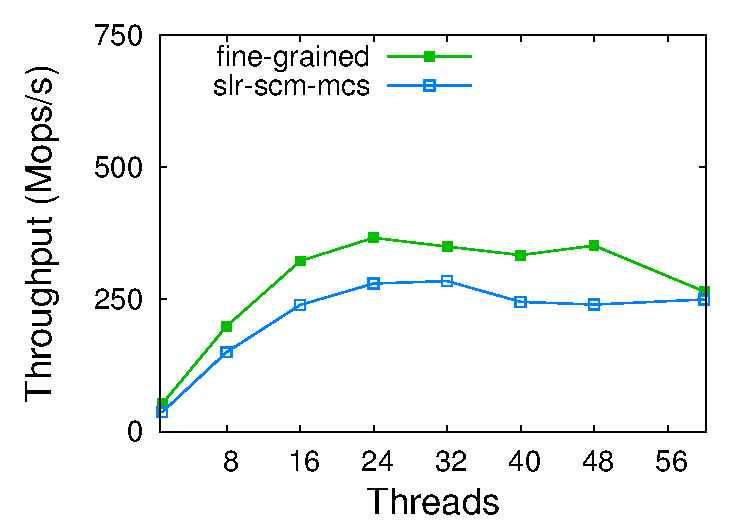
\includegraphics[width=0.45\textwidth]{Scal-u10-i1000(noset)}}
\subfigure[\textit{i} = 10$^6$]{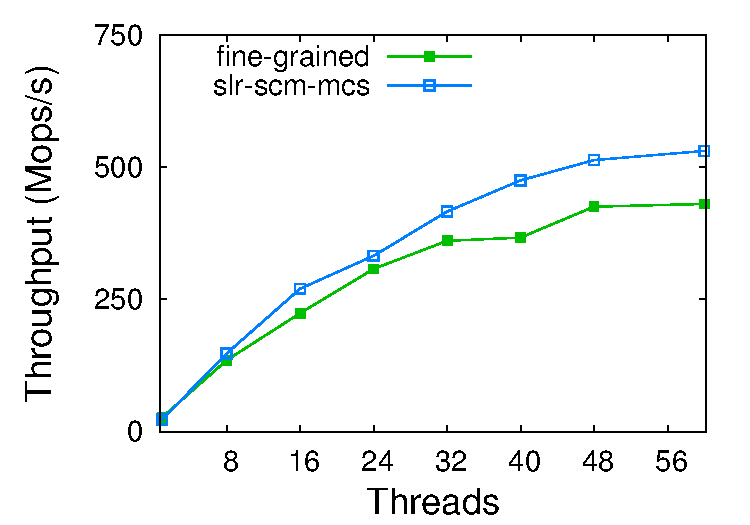
\includegraphics[width=0.45\textwidth]{Scal-u10-i1000000(noset)}}
\caption{传统细粒度锁方法和基于RTM的粗粒度锁方法之间的性能比较}
\label{fig:htm_coarse_grained}
\end{figure}

\textbf{分析}: 根据实验结果,总结了两点认识。
第一,在处理大规模工作集时,使用HTM构建并发哈希表的好处体现在两个方面:一是获得的性能和扩展性具有一定的竞争力;二是它能降低内存开销并达到简化并行编程的目的。
第二,当工作集的大小小于片上缓存的容量时,此时由于更加激烈的数据冲突引发频繁的事务中止影响了基于HTM的全局锁性能。

\subsection{不同的全局锁方案之间的比较}
\label{sec:htm_global}
进一步的评估使用不同的锁实现方式作为全局锁之间的性能差异。
为此实现了6种锁方法,它们分别是:
(1)标准的MCS锁,没有使用任何优化的MCS锁方法;
(2)用SLR优化的基于HTM的MCS锁(slr-mcs);
(3)基于HTM的事务重试方法(HTM-retry);不使用SLR和SCM进行优化,仅参照Intel技术手册上推荐的方法对发生中止的事务进行重试,重试的次数设定为10。
(4)使用SCM优化的基于HTM的ttas锁;
(5)采用SLR和SCM两种软件辅助方法共同优化的MCS锁(slr-scm-mcs);
(6)基于乐观的SCM方案的ttas锁,线程在经过10次重试事务执行后仍无法成功提交时,线程会以事务性的方式获取锁,完成本次操作。

图~\ref{fig:htm_global}~展示了运行初始化大小为1000和1百万两个级别的工作集的性能曲线。
\begin{figure}[htbp]
\centering
%\subfigure[Intel]{
\subfigure[\textit{i} = 10$^3$]{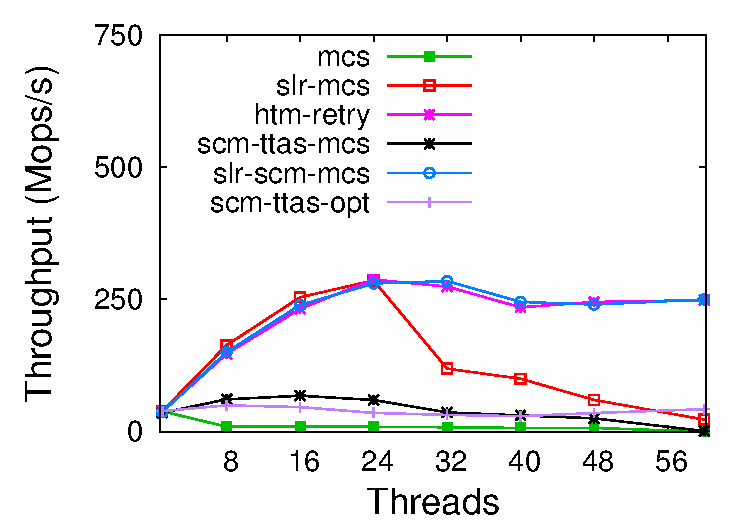
\includegraphics[width=0.45\textwidth]{coarse-grained-u10-i1000(noset)}}
\subfigure[\textit{i} = 10$^6$]{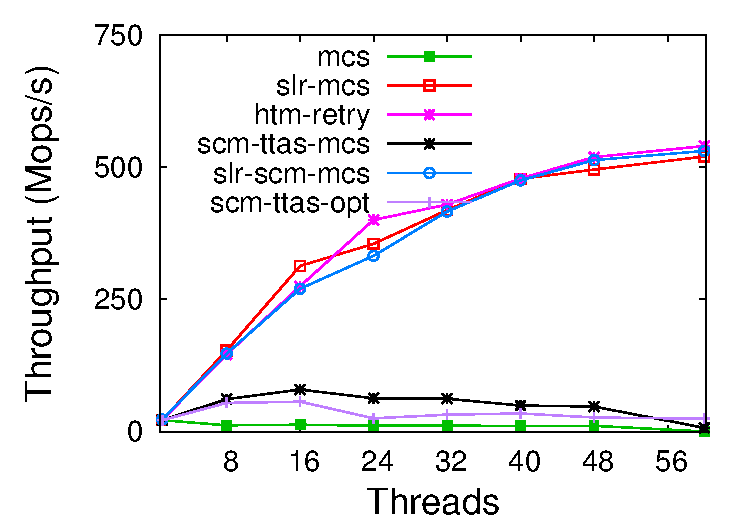
\includegraphics[width=0.45\textwidth]{coarse-grained-u10-i1000000(noset)}}
\caption{使用不同全局锁方法之间的性能比较}
\label{fig:htm_global}
\end{figure}
正如预期那样,使用传统的未经优化的MCS锁方法不论是线程扩展性还是性能都是集中方案种最差的。
从图~\ref{fig:htm_global}~(a)和(b)观察发现,当运行较小的工作集(初始化元素个数为1000)时,
slr-mcs,slr-scm-mcs和HTM-retries在\textit{n}为24时达到吞吐量峰值,之后吞吐量随着\textit{n}的增加而减少。
而其它两种方法,scm-ttas-mcs和scm-ttas-opt对应的性能只略微的比使用传统的MCS锁好一些。
在处理小规模数据时CLHT遭遇性能下降,原因是这种情况下触发数据竞争的概率是成倍增加的。
当数据集的大小超过最后一级缓存的容量时,slr-mcs, slr-scm-mcs以及HTM-retry三种方法都展现了近线性的线程扩展性。

在进行实验分析时还发现基于HTM实现的全局锁方法的CLHT的性能与线程绑定方式(三种线程绑定方式见~\ref{sec:thread_pinning}~)的影响。
这里采用紧凑型线程绑定方式。
图~\ref{fig:htm_pinning}~中描述了本次实验的结果。
\begin{figure}[htbp]
\centering
%\subfigure[Intel]{
\subfigure[\textit{i} = 10$^3$]{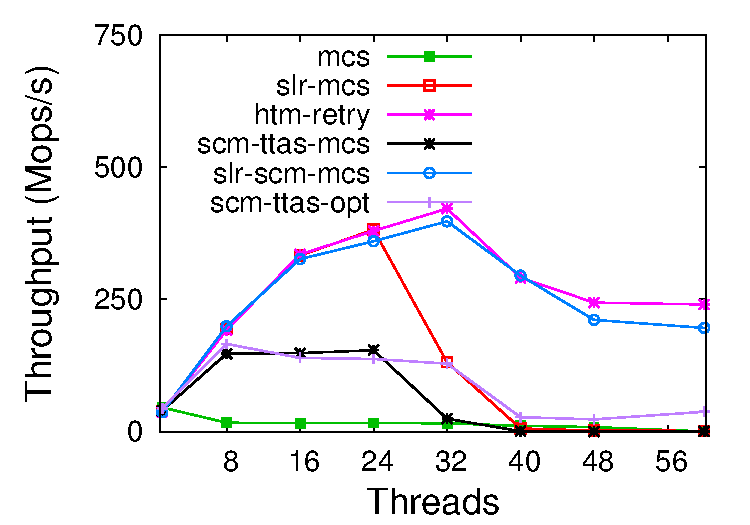
\includegraphics[width=0.45\textwidth]{coarse-grained-u10-i1000(setcpu)}}
\subfigure[\textit{i} = 10$^6$]{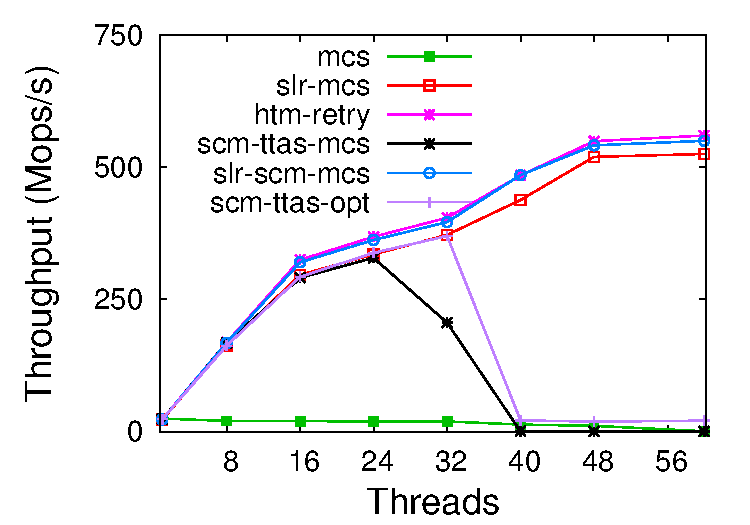
\includegraphics[width=0.45\textwidth]{coarse-grained-u10-i1000000(setcpu)}}
\caption{紧凑型线程绑定方案运行结果}
\label{fig:htm_pinning}
\end{figure}
通过与图~\ref{fig:htm_global}~的比较,有两个方面的发现:
其一,slr-scm-mcs, slr-mcs和HTM-retry三种方案的受线程绑定方式的影响较小,并且比其它几种方案的性能更加稳定。
其二,scm-ttas-mcs和scm-ttas-opt在单个socket内表现出较好的扩展性,然而当线程数量超过单个socket能够提供的最大线程数量时,它们的性能下降严重。
这种现象是由于它们在NUMA架构下,跨插槽通信的能力较弱引起的。

在~\ref{sec:htm_analysis}~中,将通过测算总的事务量、事务中止率以及发起锁请求的次数三个指标具体分析引起不同线程绑定方式之间性能差异的原因。

\textbf{分析}:从这一部分的实验中,得到的结论分为三个方面:
一是,MCS和HTM-retry同样是使用全局锁,后者是基于HTM的方法,未使用任何软件优化方案,两者之间的性能差异巨大,验证了硬件事务内存有助于激发多核处理器性能的说法;
二是,使用基于HTM实现的锁方法,能够在性能上有多大的提升取决于所使用的软件辅助优化技术;
第三,slr-scm-mcs和HTM-retry两种方案在扩展性上较其它方法更具有竞争力。


\subsection{基于HTM的细粒度锁实现与传统细粒度方法的比较}
使用基于HTM的全局锁构建并发哈希表有利于性能的提升。
还有一个令人关心的问题,如果使用基于HTM实现的锁用于构建并发哈希表会对性能提升有帮助吗?
下面将通过实验来回答这个问题。

参照实现基于HTM的粗粒度CLHT的实现方法实现了基于HTM的细粒度锁方法,并将其与原作者实现的细粒度版本在相同的测试平台上处理同样的工作集。
运行结果如图~\ref{fig:htm_fine_grained}~所示。
\begin{figure}[htbp]
\centering
%\subfigure[Intel]{
\subfigure[\textit{i} = 10$^3$]{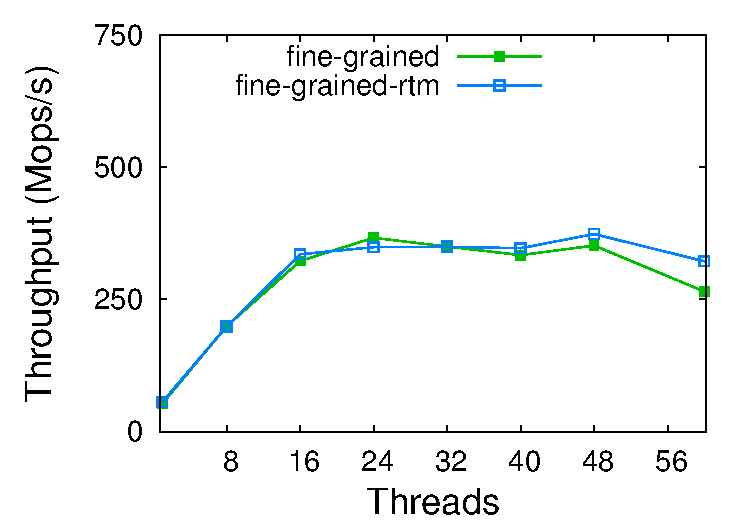
\includegraphics[width=0.45\textwidth]{fine-grained-u10-i1000}}
\subfigure[\textit{i} = 10$^6$]{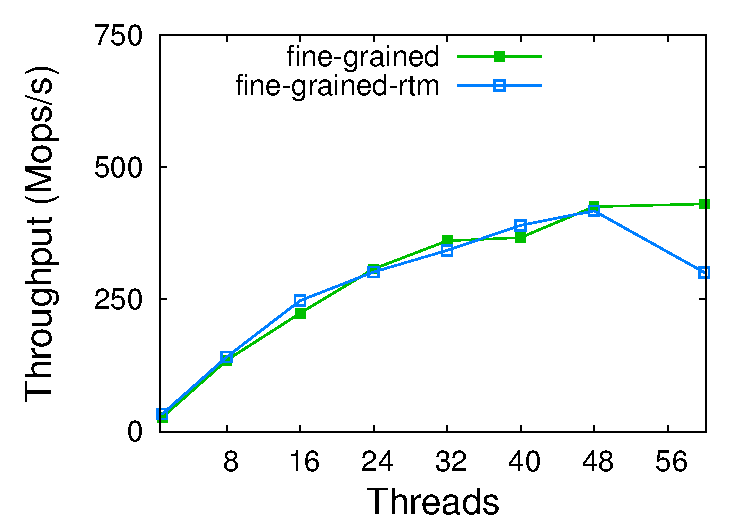
\includegraphics[width=0.45\textwidth]{fine-grained-u10-i1000000}}
\caption{使用/不使用HTM的细粒度锁方法之间的性能比较}
\label{fig:htm_fine_grained}
\end{figure}
通过比较得知,\textit{n} < 48时,两个版本间的性能差异并不明显。
产生这种现象的原因在于使用传统的细粒度的锁方法能够有效的避免在同一时刻多个线程同时访问相同内存地址。
因此,在这种情形下使用HTM对其进行优化以期获得更高性能的做法意义不大。
图~\ref{fig:htm_fine_grained}~(a)中,\textit{n} > 48时,使用HTM的CLHT的性能要略好于纯粹的细粒度锁方法。
原因是随着参与运算的线程数量的增加导致线程间的竞争更加激励,而HTM在数据冲突不是特别激烈的情况下是有利于提升并行化的。

\textbf{分析}:经过试验比较,得到的结论是:
在传统的细粒度锁方法能够提供良好的线程扩展性和性能的前提之下,使用HTM进行优化既达不到简化并发控制的目的,又对整体性能的提升没有助益。

\subsection{影响HTM性能的因素分析}
\label{sec:htm_analysis}

图~\ref{fig:htm_global}~展现了CLHT使用五个不同的基于HTM的同步方案的性能曲线,为了探究造成它们性能上的差异的原因,借助Intel的性能计数监视器(PMU)收集了一些微观的运行时指标。
这部分内容只挑选最能说明观察到的实验现象的指标予以说明。
表~\ref{tab:htm_abort_rate}~表中数据样本来自线程数为32,执行初始化大小分别为1百万/1000,更新比重为10\%的工作集。
表中第二列(c$_2$)数据表示运行中请求锁的次数,第三列(c$_3$)为发起的总的事务量,第4列(c$_4$)表示被中止的事务的数量,最后一列为中止率,通过c$_4$/c$_3$计算得到。
事务中止率\textit{r}由中止的事务量除以执行期间发起的总的事务量计算得到,总的事务量为中止的事务量与提交的事务量之和。
从表~\ref{tab:htm_abort_rate}~的数据中,观察发现不同的HTM方案对应的中止的事务量差别不大,表明中止的事务量并不是最主要的性能瓶颈,而执行中申请锁的次数以及发起的总的事务量直接对整体的性能造成影响。
申请锁的次数和提交的事务量越多,对应的吞吐量越高。
比如,slr-mcs,scm-ttas-mcs和HTM-retry对应的申请锁的次数和提交的事务量明显高于其它两种方案,正好对应图~\ref{fig:htm_global}~,这三种方法的性能曲线比另外两种更加理想。

\begin{table}[htbp]
  \centering
  \caption{Intel PMU收集的不同的HTM方法的运行时数据}
  \label{tab:htm_abort_rate}
  \begin{tabular}{ccccc}
    \toprule
                  & 申请锁的次数(百万) & 总的事务量(百万) & 中止的事务量 & 中止率(\%) \\
    \midrule
      HTM-retry   & 170/160           & 290/360         & 53/67      & 18.3/18.5 \\
      slr-mcs     & 160/60            & 290/360         & 52/67      & 18.6/18.6 \\
      slr-scm-mcs & 160/160           & 300/350         & 52/66      & 17.8/19.0 \\
      scm-ttas-mcs& 48/12             & 110/130         & 51/62      & 48.6/48.4 \\
      scm-ttas-opt& 110/48            & 220/180         & 53/65      & 23.0/35.4 \\
    \bottomrule
  \end{tabular}
\end{table}

此外,通过观察发现吞吐量随着中止率的升高而下降。
通过运行不同的参数组合来探究中止率、创建的线程的数量、更新比重以及哈希表初始化元素个数几者之间的关系。
表~\ref{tab:abort_rate_thread}~用以说明线程数与中止率之间的关系。
表~\ref{tab:abort_rate_thread}~的第二列和第三列分别表示发起的事务总量和被中止的事务量。
不论是发起的事务总量还是被中止的事务量都随着线程数量的增加而增加,然而被中止的事务量的增长速率远低于发起的事务量的增长速率。
换言之,随着越来越多的线程被创建用来参与运算,被提交的事务量的增长远远大于被中止的事务量的增长。
这个趋势与图~\ref{fig:htm_fine_grained}~中的线程的线程扩展性曲线相符合。

\begin{table}[htbp]
  \centering
  \caption{slr-scm-mcs方案的中止率随线程变化情况}
  \label{tab:abort_rate_thread}
  \begin{tabular}{cccc}
    \toprule
      \textit{n}  & 总的事务量(百万) & 中止的事务量 & 中止率(\%) \\
    \midrule
      2   & 156/156 & 70/66 & 43.6/42.3  \\
      8   & 228/239 & 72/59 & 31.6/21.5 \\
      16  & 303/298 & 73/64 & 24.1/19.5  \\
      32  & 382/349 & 80/67 & 20.9/19.2  \\
      40  & 399/299 & 77/74 & 19.3/24.8 \\
      48  & 495/310 & 87/78 & 17.6/25.2  \\
      64  & 522/316 & 90/89 & 17.2/26.0 \\
    \bottomrule
  \end{tabular}
\end{table}

表~\ref{tab:htm_update}~中的数据用以说明中止率随工作集中更新比重的变化情况。
线程数为32,表的第2到第4列表示的内容与表~\ref{tab:htm_abort_rate}~相同,每一列表中记录了两组数据,分别代表初始化值为1百万和1000时的测试结果。
这一次,运行的测试集中更新比重分别为0,10和80。
实验获得的结果是,运行不包含更新操作的工作集,对应的中止率也最低。
这是因为在纯读的场景下,没有写入内存的请求,这样发生数据冲突的概率很小,从而引起的事务中止也相对较少。
随着更新比重的增加,中止率会上升,随之而来的是性能的下降。

\begin{table}[htbp]
  \centering
  \caption{slr-scm-mcs方案的中止率随更新比重变化情况}
  \label{tab:htm_update}
  \begin{tabular}{cccc}
    \toprule
      \textit{n}  & 总的事务量(百万) & 中止的事务量 & 中止率(\%) \\
    \midrule
      0   &  346/554 & 73/60 & 21.1/10.8  \\
      10  &  320/352 & 70/66 & 21.9/18.8 \\
      80  &  282/273 & 74/70 & 26.4/25.6  \\
    \bottomrule
  \end{tabular}
\end{table}

\section{本章小结}
本章首先对事务内存、Intel TSX提供的两种接口——HLE和RTM——进行了介绍。提出了针对Intel TSX的两种软件优化方法:SLR和SCM。

然后,从对哈希表串行执行五次操作的实例入手,由浅入深的探讨了当前主流的三种同步锁模型:粗粒度锁,细粒度锁和硬件事务内存,在构建并发哈希表上的优势和劣势。
粗粒度锁方法实现简单,易于理解,且容易保障正确性,但是使用这种方法获得的性能很不理想。
细粒度锁方法能够发挥出多核系统的性能优势,并且有很好的线程扩展性,但是细粒度锁增加了设计并发哈希表的难度,并且需要花费大量精力在保证正确性上。
事务内存继承前两者的优势于一身,实现简单,易于验证正确性,又能够获得接近甚至超越细粒度锁方案的性能,是理想的并发编程范式。

接着,以基于细粒度锁的缓存行哈希为蓝本,使用SLR和SCM实现了基于硬件事务内存的并发哈希表,并就二者的性能进行了比较,证明了基于HTM的并发哈希表能够保证良好的线程扩展性和性能,并且在工作集较大的场景下,性能比细粒度锁实现更优。

实现了6种不同的粗粒度并发哈希,用于进一步的探究使用哪一种方法对基于HTM的并发哈希表的优化粒度更大。
并通过实验表明,在细粒度锁方案已经能够保证良好的性能和线程扩展性的前提下,使用HTM优化细粒度锁方案对于性能的提升没有意义。

最后,影响硬件事务内存性能发挥的因素进行了分析。通过测算测试过程中发起的事务总量、被中止的事务量以及中止率对实验评估中的一些现象进行解释说明。

对基于硬件事务内存的并发哈希表的评估结果表明,本章提出的方法达到了预期目标。
对于并发哈希表的设计具有重要的意义。
